% ============================================================
% Lecture 10 -- Problem of parameter estimation
% ============================================================
\section{The Problem of Parameter Estimation}\label{sec:L10}

\lectureheader{10}{TnJ_1LZXLBk}{Week-3 handwritten notes \texttt{Feb9.pdf}, part ``The problem of estimation of the parameters'' (linear parametric functions, estimability theorem); Week-5 assignment Q2, Q5, Q6}

\begin{guiding*}
By the end of this lecture you should be able to:
\begin{itemize}
  \item define a \emph{linear parametric function} $\lambda\T\beta$ and say when it is \emph{estimable};
  \item prove that $\lambda\T\beta$ is estimable if and only if $\lambda\in\colsp{X\T}$;
  \item decide estimability in concrete models, including the one-way classification;
  \item relate estimability to the null space of $X$ and to identifiability.
\end{itemize}
\end{guiding*}

\subsection{Recap}
In the linear model $(Y,X\beta,\sigma^2I_n)$ of \cref{sec:L09}, the unknown parameters are
$\beta\in\RR^p$ and $\sigma^2>0$, i.e.\ $(\beta,\sigma^2)\in\RR^p\times\RR_+$. In
\cref{sec:L08} we saw that in the one-way model some linear combinations of $\beta$ (such as
$\mu_1-\mu_2$) have unbiased estimates, while others (such as $\mu$) cannot even be identified.
This lecture characterises the good combinations.

\subsection{Linear parametric functions}
\begin{definition}[Linear parametric function]\label{def:L10-lpf}
For $\lambda=(\lambda_1,\dots,\lambda_p)\T\in\RR^p$, the linear combination
\[
\lambda\T\beta=\lambda_1\beta_1+\lambda_2\beta_2+\dots+\lambda_p\beta_p
\]
of the parameter vector is called a \vocab{linear parametric function}.
\end{definition}
In a linear model we will be interested only in linear parametric functions. The instructor
writes $p\T\beta$ with $p\in\RR^m$; we write $\lambda\T\beta$ because $p$ denotes the number of
parameters in this book.

\begin{definition}[Estimable]\label{def:L10-estimable}
Let $(Y,X\beta,\sigma^2I_n)$ be a linear model and $\lambda\in\RR^p$. The linear parametric function
$\lambda\T\beta$ is \vocab{estimable} if there exists $\ell\in\RR^n$ such that
\[
\EE[\ell\T Y]=\lambda\T\beta\qquad\text{for every }\beta\in\RR^p .
\]
In other words, $\lambda\T\beta$ is estimable if it has a \emph{linear unbiased estimate} $\ell\T Y$.
\end{definition}
Unbiasedness must hold for every value of $\beta$. An estimate that is unbiased only for some
$\beta$'s is useless, because we do not know $\beta$.

\subsection{The estimability theorem}
\begin{theorem}[Characterisation of estimability]\label{thm:L10-estimable}
Let $(Y,X\beta,\sigma^2I_n)$ be a linear model and $\lambda\in\RR^p$. Then
\[
\lambda\T\beta \text{ is estimable}\iff \lambda\in\colsp{X\T},
\]
where $\colsp{X\T}=\{z\in\RR^p:\ z=X\T\ell\text{ for some }\ell\in\RR^n\}$ is the column space of
$X\T$, which is the row space of $X$.
\end{theorem}
\begin{proof}
We follow the chain of equivalences in the notes and justify each step.
\begin{align*}
\lambda\T\beta\text{ estimable}
&\iff \exists\,\ell\in\RR^n:\ \EE[\ell\T Y]=\lambda\T\beta\ \ \forall\beta\in\RR^p &&\text{(definition)}\\
&\iff \exists\,\ell\in\RR^n:\ \ell\T X\beta=\lambda\T\beta\ \ \forall\beta\in\RR^p &&\text{(linearity of expectation)}\\
&\iff \exists\,\ell\in\RR^n:\ X\T\ell=\lambda &&\text{(linear algebra, below)}\\
&\iff \lambda\in\colsp{X\T}. &&\text{(definition of column space)}
\end{align*}
Step 2: $\EE[\ell\T Y]=\ell\T\EE[Y]=\ell\T X\beta$ by \cref{prop:L09-rules}.
Step 3: $\ell\T X\beta=\lambda\T\beta$ for all $\beta$ means $(X\T\ell-\lambda)\T\beta=0$ for all $\beta$.
Taking $\beta=X\T\ell-\lambda$ gives $\pnorm{X\T\ell-\lambda}^2=0$, i.e.\ $X\T\ell=\lambda$. Conversely,
if $X\T\ell=\lambda$ then $\ell\T X\beta=(X\T\ell)\T\beta=\lambda\T\beta$ for all $\beta$.
\end{proof}

\begin{note}
The proof shows more than the statement. The linear unbiased estimates of $\lambda\T\beta$ are
\emph{exactly} the $\ell\T Y$ with $X\T\ell=\lambda$ (this is Week-5 assignment Q2). If some
$\ell_0$ works, then so does $\ell_0+v$ for every $v\in\nullsp{X\T}$. So there are usually many
linear unbiased estimates, and the question ``which one is best?'' (Weeks~5--6) makes sense.
\end{note}

\begin{corollary}\label{cor:L10-fullrank}
Every linear parametric function is estimable $\iff\colsp{X\T}=\RR^p\iff\rank(X)=p$.
In that case the parameters $\beta_1,\dots,\beta_p$ themselves are estimable.
\end{corollary}
\begin{proof}
All $\lambda$ lie in $\colsp{X\T}$ iff $\colsp{X\T}=\RR^p$, i.e.\ iff $\dim\colsp{X\T}=\rank(X)=p$.
Then $\beta_j=e_j\T\beta$ is estimable for each standard basis vector $e_j$.
\end{proof}

\begin{corollary}[Estimable functions form a subspace]\label{cor:L10-subspace}
If $\lambda_1\T\beta$ and $\lambda_2\T\beta$ are estimable, so is $(a\lambda_1+b\lambda_2)\T\beta$ for all
$a,b\in\RR$. Each row $x_i\T\beta=\EE Y_i$ of $X\beta$ is estimable (take $\ell=e_i$). Every estimable
function is a linear combination of these.
\end{corollary}
\begin{proof}
$\colsp{X\T}$ is a subspace spanned by the rows $x_1,\dots,x_n$ of $X$. If
$\lambda_1=X\T\ell_1$ and $\lambda_2=X\T\ell_2$ then $a\lambda_1+b\lambda_2=X\T(a\ell_1+b\ell_2)$.
\end{proof}

\begin{proposition}[Week-5 assignment Q5]\label{prop:L10-nullspace}
$\lambda\T\beta$ is estimable $\iff$ $\lambda$ is orthogonal to the null space $\nullsp{X}=\{v:Xv=0\}$.
\end{proposition}
\begin{proof}
By \cref{thm:L10-estimable} we must show $\colsp{X\T}=\nullsp{X}^\perp$.
($\subseteq$) If $\lambda=X\T\ell$ and $Xv=0$, then $\lambda\T v=\ell\T Xv=0$.
($\supseteq$) Both are subspaces of $\RR^p$. $\dim\colsp{X\T}=\rank(X)=r$, and by rank--nullity
$\dim\nullsp{X}=p-r$, so $\dim\nullsp{X}^\perp=r$. A subspace contained in another of the same
finite dimension equals it.
\end{proof}

\begin{note}[Supplementary: estimable $\Rightarrow$ identifiable]
If $\lambda\T\beta$ is estimable and $X\beta_1=X\beta_2$, then $\beta_1-\beta_2\in\nullsp{X}$, so
$\lambda\T\beta_1=\lambda\T\beta_2$ by \cref{prop:L10-nullspace}. Estimable functions are therefore
identifiable in the sense of \cref{def:L08-ident}. Conversely, a linear function that is
identifiable (constant on each set $\{\beta: X\beta=\text{const}\}$) must vanish on $\nullsp{X}$, so it
is estimable. For linear parametric functions the two notions coincide.
\end{note}

\subsection{Examples}
\begin{example}[One-way model with $k=2$, $n_1=n_2=2$]\label{ex:L10-oneway}
With $\beta=(\mu,\mu_1,\mu_2)\T$ and $Y=(Y_{11},Y_{12},Y_{21},Y_{22})\T$,
\[
X=\begin{pmatrix}1&1&0\\1&1&0\\1&0&1\\1&0&1\end{pmatrix},\qquad
\colsp{X\T}=\mathrm{span}\{(1,1,0)\T,(1,0,1)\T\}.
\]
\begin{itemize}
  \item $\mu_1-\mu_2$: $\lambda=(0,1,-1)\T=(1,1,0)\T-(1,0,1)\T\in\colsp{X\T}$, so it is \emph{estimable}. Two linear unbiased estimates are $\ell=(1,0,-1,0)\T$, i.e.\ $Y_{11}-Y_{21}$, and $\ell=(\tfrac12,\tfrac12,-\tfrac12,-\tfrac12)\T$, i.e.\ $\bar Y_{1\cdot}-\bar Y_{2\cdot}$. Both satisfy $X\T\ell=(0,1,-1)\T$. Their variances are $\sigma^2\pnorm{\ell}^2=2\sigma^2$ and $\sigma^2$ respectively.
  \item $\mu+\mu_1$: $\lambda=(1,1,0)\T$ is a row of $X$, so it is \emph{estimable} (e.g.\ by $Y_{11}$, or better by $\bar Y_{1\cdot}$).
  \item $\mu_1$: $\lambda=(0,1,0)\T$. If $a(1,1,0)+b(1,0,1)=(0,1,0)$ then $a+b=0$, $a=1$, $b=0$, a contradiction. So it is \emph{not estimable}. Equivalently, $\nullsp{X}=\mathrm{span}\{(1,-1,-1)\T\}$ and $\lambda\T(1,-1,-1)\T=-1\ne0$.
  \item $\mu$: $\lambda=(1,0,0)\T$ has $\lambda\T(1,-1,-1)\T=1\ne 0$, so it is \emph{not estimable}.
\end{itemize}
\end{example}

\begin{example}[General one-way model]\label{ex:L10-oneway-general}
In Model~1 with $\beta=(\mu,\mu_1,\dots,\mu_k)\T$, the rows of $X$ are $(1,e_i\T)$. By
\cref{prop:L08-rank}, $\nullsp{X}$ is one-dimensional, spanned by $v=(1,-1,\dots,-1)\T$.
Hence, by \cref{prop:L10-nullspace},
\[
\lambda_0\mu+\sum_{i=1}^k\lambda_i\mu_i\ \text{is estimable}\iff \lambda_0=\sum_{i=1}^k\lambda_i .
\]
Consequences: any \vocab{contrast} $\sum\lambda_i\mu_i$ with $\sum\lambda_i=0$ is estimable (e.g.\
$\mu_1-\mu_2$, $\mu_1+\mu_2-2\mu_3$), and so is $\mu+\mu_i$. The functions $\mu$ and $\mu_i$ alone are not.
This answers \cref{q:L08-questions}.
\end{example}

\begin{figure}[ht]
\centering
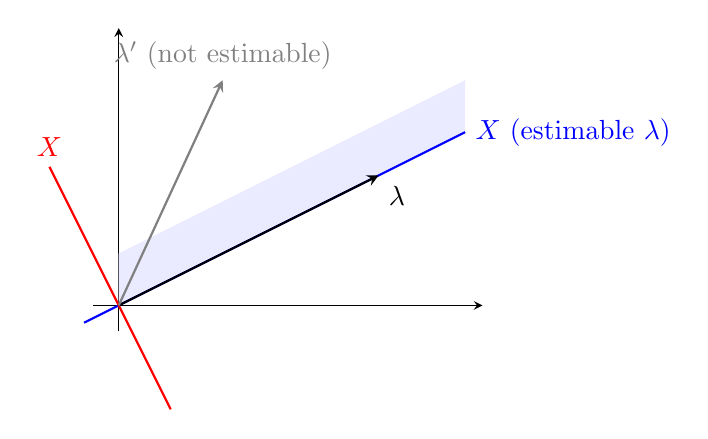
\begin{tikzpicture}[scale=1.1,>=stealth]
\draw[->] (-0.3,0) -- (4.2,0) node[right] {};
\draw[->] (0,-0.3) -- (0,3.2);
\fill[blue!8] (0,0) -- (4,2) -- (4,2.6) -- (0,0.6) -- cycle;
\draw[thick,blue] (-0.4,-0.2) -- (4,2) node[right] {$\colsp{X\T}$ (estimable $\lambda$)};
\draw[thick,red] (0.6,-1.2) -- (-0.8,1.6) node[above] {$\nullsp{X}$};
\draw[->,thick] (0,0) -- (3,1.5) node[below right] {$\lambda$};
\draw[->,thick,gray] (0,0) -- (1.2,2.6) node[above] {$\lambda'$ (not estimable)};
\end{tikzpicture}
\caption{$\lambda\T\beta$ is estimable exactly when $\lambda$ lies in the row space $\colsp{X\T}=\nullsp{X}^\perp$ (schematic, $p=2$, $\rank X=1$).}
\label{fig:L10-geom}
\end{figure}

\subsection{Computation}
To test whether $\lambda\in\colsp{X\T}$ numerically, compare $\rank(X\T)$ with $\rank([X\T\ \lambda])$,
or check whether $\lambda$ is orthogonal to a basis of $\nullsp{X}$ (\texttt{scipy.linalg.null\_space}).
A third test uses the Moore--Penrose inverse: $\lambda\in\colsp{X\T}\iff X\T(X\T)^{+}\lambda=\lambda$.
All three are implemented, and checked on \cref{ex:L10-oneway}, in
\nb{week03/L10\_estimability.ipynb}. The notebook also finds $\ell$ with $X\T\ell=\lambda$ and
verifies unbiasedness by simulation.

\subsection{Summary}
\begin{itemize}
  \item Linear parametric function: $\lambda\T\beta$. Estimable: $\exists\,\ell$ with $\EE[\ell\T Y]=\lambda\T\beta$ for all $\beta$.
  \item \textbf{Theorem:} $\lambda\T\beta$ is estimable $\iff\lambda\in\colsp{X\T}\iff\lambda\perp\nullsp{X}$. The linear unbiased estimates are $\ell\T Y$ with $X\T\ell=\lambda$.
  \item If $\rank X=p$, everything is estimable. Estimable functions form the $r$-dimensional space spanned by the rows of $X$.
  \item One-way model: $\lambda_0\mu+\sum\lambda_i\mu_i$ is estimable iff $\lambda_0=\sum\lambda_i$.
\end{itemize}

\subsection{Exercises}
\begin{problem}\label{prob:L10-1}
In the one-way model with $k=3$, decide which are estimable: $\mu$, $\mu_1-\mu_2$, $\mu+\mu_1$, $\mu_1+\mu_2-2\mu_3$, $2\mu+\mu_1+\mu_2$.
\end{problem}
\begin{problem}\label{prob:L10-2}
(Week-5 assignment Q6.) Let $k,l\ge 2$ be integers and let $X$ have rows $(1,i,ik)$ for $i=1,\dots,k$ followed by rows $(1,i,il)$ for $i=1,\dots,l$, with $\beta=(\beta_1,\beta_2,\beta_3)\T$.
(a) Show that $\beta_1$ and $\beta_2+\beta_3(l+k)/2$ are always estimable.
(b) Find a necessary and sufficient condition on $k,l$ for every linear function of $\beta$ to be estimable.
\end{problem}
\begin{problem}\label{prob:L10-3}
Show that if $\lambda\T\beta$ is estimable, then any two linear unbiased estimates $\ell_1\T Y,\ell_2\T Y$ differ by $v\T Y$ with $v\in\nullsp{X\T}$, and that $\EE[v\T Y]=0$.
\end{problem}
\begin{problem}\label{prob:L10-4}
In simple linear regression $Y_i=\beta_1+\beta_2x_i+\eps_i$, when is $\beta_2$ estimable? Relate your answer to \cref{prob:L05-4}.
\end{problem}
\begin{problem}\label{prob:L10-5}
In the nested model of \cref{ex:L09-nested-mat}, show that $\delta_{11}-\delta_{12}$ is estimable but $\mu_1-\mu_2$ is not.
\end{problem}

\subsection{Further reading}
Christensen, \S2.1 (Identifiability and Estimability), especially the result that $\lambda\T\beta$
is estimable iff $\lambda\T=\rho\T X$ for some $\rho$. Rao, \S4a.1 (estimable parametric functions).
